\chapter{nHCal}\label{cha:nHCal} % chktex 24
extensively from pre-TDR - new iteration in two weeks - is it worth the wait? \textit{probably not}

WHERE IS THE GOOGLE DOC? is this it? \url{https://docs.google.com/document/d/1WBacN4zQDPq5SoQz7Dx542Mwn0gY34H2S_qPBLp2SVQ/edit?tab=t.0#heading=h.3hyq6s4efrbn}

\section{Motivation}
tail catcher of nECal

start with HERA (maybe) - then continue from that ("to not make the same mistake")

Vector meson - the matrix image \ref{fig:nhcal:K1K2matica} + the 012K plots \ref{fig:nhcal:e+Au-phi(KK)}

should I only be mentioning this for e + Au and phi, or also e + p, and J/psi?
\\\,\\
\textbf{the original [JLab] requirements still valid}

Backward HCal shall provide functionality of a tail catcher for the high resolution e/m calorimeter in electron identification, as well as for jet kinematics measurement at small Bjorken x

Shall accommodate the possibility of hadron energy measurements in the range up to few dozens of GeV and pseudorapidity down to -3.5

Must provide capability to cover pseudo rapidity range down to at least -3.5.

Shall accommodate the ability to complement e/m calorimeter by tail catching capability for electron ID purposes, especially below 3-4 GeV/c.

Shall provide capability to have energy resolution s(E)/E ~ 100\%/sqrt(E) + a 10\% constant term.

Must provide space to have tower depth of 3-4 interaction lengths (together with the e/m PWO crystal calorimeter) in order to suppress longitudinal leakage for relatively small hadron energies in the e-endcap.

Should be built of non-magnetic materials

Shall not interfere with the detector solenoid magnetic field


\section{Construction}
realistic dimensions and location

tiling? is it really important?

does clustering make sense to mention? - probably somewhere else (simulations)

changes?:

sampling fraction - possible to be compensating (Elke says NO)? what did Subhadip prove, then? - how achieved? how calculated?

but what about true construction? does Leszek now? does anybody?

two images from BP? or something else? cite myself?

anything about neutrons? meaningful?

\section{?}
is tilt usable? if for VU, also for DP?

\section{answers}

MATERIAL:
really non-magnetic steel material="StainlessSteelSAE304"\\
material name="StainlessSteelSAE304"
type="density" value="7.9" unit="g / cm3"
fraction n="0.74" ref="Fe"/
fraction n="0.18" ref="Cr"/
fraction n="0.08" ref="Ni"/

material name="Polystyrene"\\
value="1.032" unit="g/cm3"
composite n="19" ref="C"
composite n="21" ref="H"
name="BirksConstant" value="0.126*mm/MeV"\\
\url{https://en.wikipedia.org/wiki/Birks%27_law} \textit{worth a mention?}


\begin{figure}[H]
    \centering
    \begin{subfigure}{.48\linewidth}
        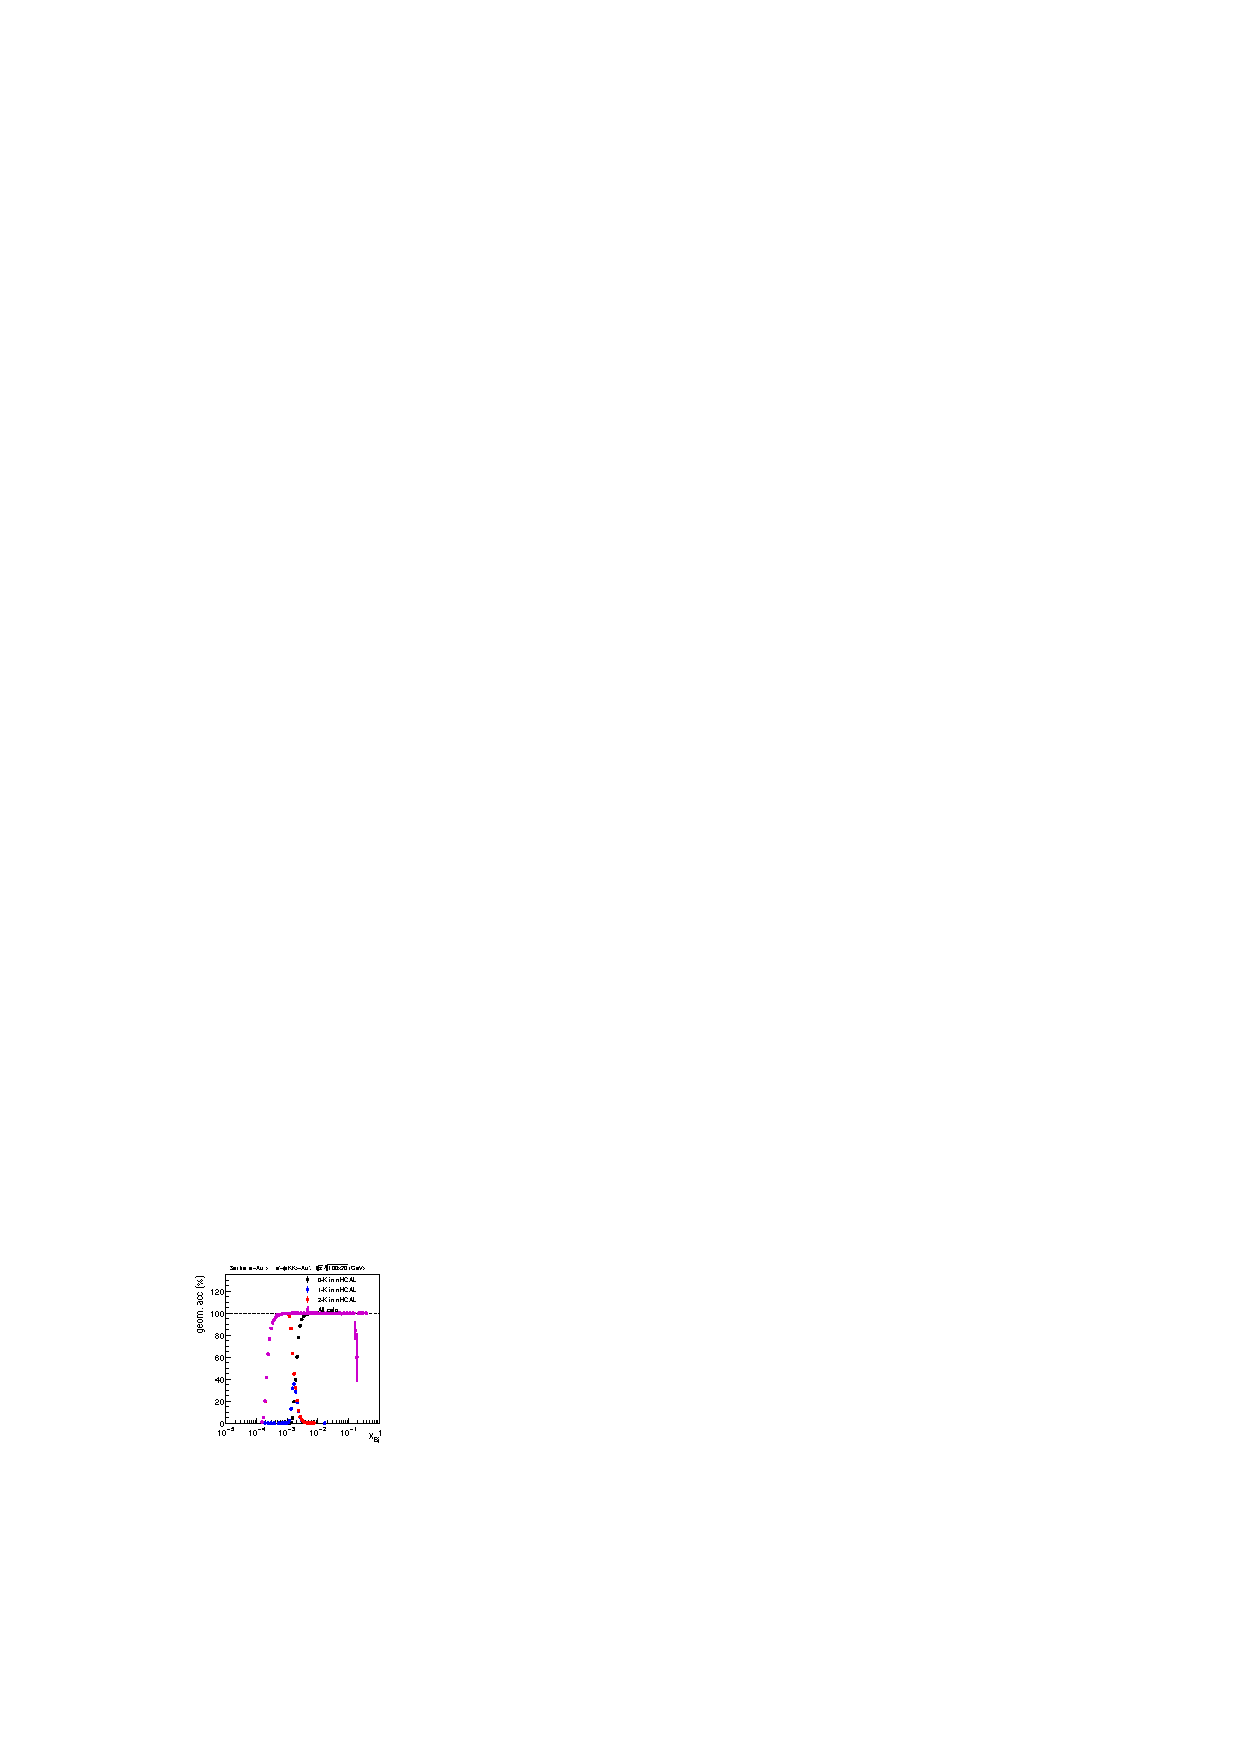
\includegraphics[width=.95\linewidth]{img/e+Au-phi(KK).pdf}
        \caption{[Caroline paper]}
        \label{fig:nhcal:e+Au-phi(KK)}
    \end{subfigure}
    \begin{subfigure}{.48\linewidth}
        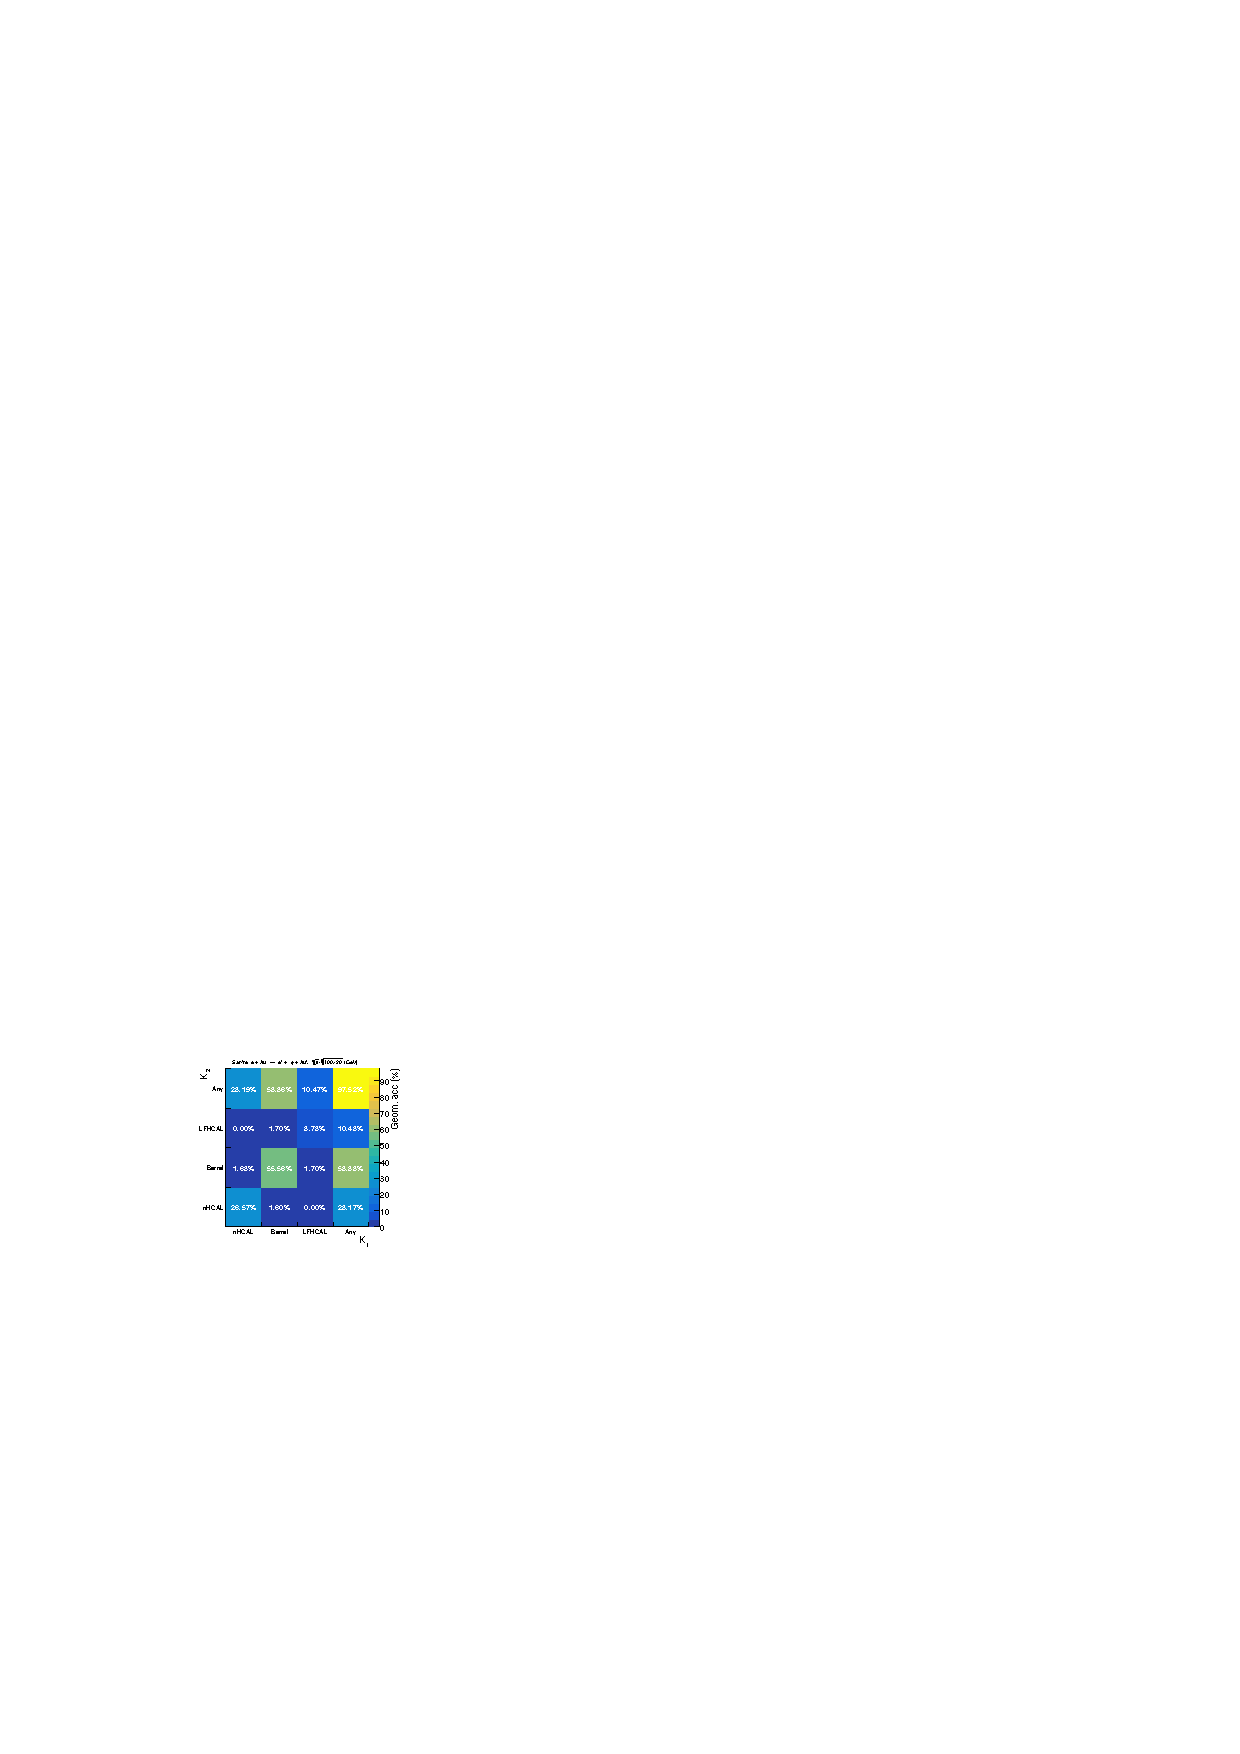
\includegraphics[width=\linewidth]{img/K1K2matica.pdf}
        \caption{[Caroline paper]}
        \label{fig:nhcal:K1K2matica}
    \end{subfigure}
\end{figure}
